\documentclass{article}

\usepackage[T1]{fontenc}
\usepackage[utf8]{inputenc}
\usepackage[french,english]{babel}
\usepackage{graphicx}
\usepackage{hyperref}
\usepackage{listings}
\usepackage{minted}
\usepackage{amsmath}
\usepackage[bottom=2.0cm,top=2.0cm,left=2.0cm,right=2.0cm]{geometry}

\title{Rapport intermédiaire \\ pour le projet long : Guess The IA}

\author{Thomas Bignon, Laura Wang}

\date{Rendu le 18 Février 2022}

\begin{document}

\maketitle

\selectlanguage{french}

\section{Présentation générale du projet}

\subsection{Description simple}

Le projet est un jeu, sous forme de page web, pouvant être joué de 2 à 4 joueurs. En se connectant, les joueurs devront choisir un pseudo et éventuellement sélectionner une photo de profil parmi une collection. Ensuite, ils auront le choix entre créer un salon ou rejoindre un salon avec un code. Un des joueurs va créer un "salon", potentiellement paramétrer la partie (sélectionner le nombre de joueurs ou de manche), puis récupérer un code, permettant aux autres joueurs de le rejoindre grâce au code. Une fois que tout le monde a rejoint, le joueur ayant créé le salon peut lancer la partie. Une partie pourra se dérouler en une ou plusieurs manches.

\paragraph{Partie 1} Une manche se déroule en deux parties. La première partie est la partie de dessin. Tous les joueurs vont voir s'afficher sur leur écran un même mot décrivant ce qu'il faut dessiner et un espace de dessin blanc. Pour dessiner, le joueur aura accès à un outil pinceau simple, de couleur noire et un outil gomme pour effacer ses traits. Une fois 10 secondes passées, le temps de dessin est écoulé.

\paragraph{Partie 2}  La deuxième partie est la partie d'attribution des dessins. Sur la page de chaque joueur, les dessins des autres joueurs ainsi que le sien sera affiché. De plus, 1 à 2 dessins (en fonction du nombre de joueurs) seront générés par le site et ajoutés parmi les dessins des joueurs. Pour chaque dessin, le joueur aura le choix de l'attribuer à l'un des joueurs ou alors à l'IA (en effet, on considère que c'est une IA qui essaye de se "cacher" parmi les joueurs et essaye de se faire passer pour un joueur humain). Le joueur pourra ensuite valider son choix avant le temps imparti (non déterminé pour le moment).

\paragraph{Score et classement} Une fois toutes les manches finies, un score et un classement sera attribué à chaque joueur et afficher sur l'écran. Le score sera un total du score de chaque manche. Pour chaque manche, le score sera la somme du score de chaque partie. Pour la première partie, on donnera un score en fonction de la certitude de la reconnaissance par un modèle de reconnaissance d'image. Plus simplement, plus le modèle reconnait que le dessin est proche du mot donné, plus le joueur aura un score élevé. Cela force les joueurs à ne pas dessiner n'importe quoi pour brouiller les autres joueurs. Pour la deuxième partie, on donnera des points pour chaque bon couple dessin + joueur. Dans le cas où un joueur a attribué le dessin d'un joueur à un autre, il ne gagne pas de point. Enfin, dans le cas où un joueur attribue un dessin généré par l'IA à un autre joueur, alors il perd (relativement beaucoup - le but du jeu est bien de ne pas se faire avoir par l'IA) des points. Le but est bien évidement d'être le plus haut dans le classement en ayant le score le plus élevé, les "IAs" n'ont pas de score ni de place dans le classement.

\subsection{Description technique}

\subsubsection{Site Web et serveur}

Le serveur du site web sera un projet sous l'environnement Node.js en JavaScript. Le serveur tourne grâce à \href{https://expressjs.com/}{Express.js}. Le contenu et le style du site web sera réalisé en HTML, CSS et avec la bibliothèque \href{https://getbootstrap.com/}{Bootstrap}.

\subsubsection{Dataset et modèles}

Il y aura 2 modèles : l'un qui reconnait des images, l'autre qui les génère. Les deux seront entrainés avec le dataset du projet Quick, Draw! de Google. Le  dataset de \href{https://github.com/googlecreativelab/quickdraw-dataset}{Quick Draw} est une collection de 50 millions d'images réparties en 345 catégories. Les données ont été récupérées sur le site \url{https://quickdraw.withgoogle.com/} sur lequel des joueurs dessinent des mots et aident par extension à entrainer un modèle à reconnaitre les catégories. Les données sont très facilement téléchargeables sous plusieurs formats sur \href{https://console.cloud.google.com/storage/browser/quickdraw_dataset}{Google Cloud}.

\begin{figure}[h]
\hrulefill
\begin{center}
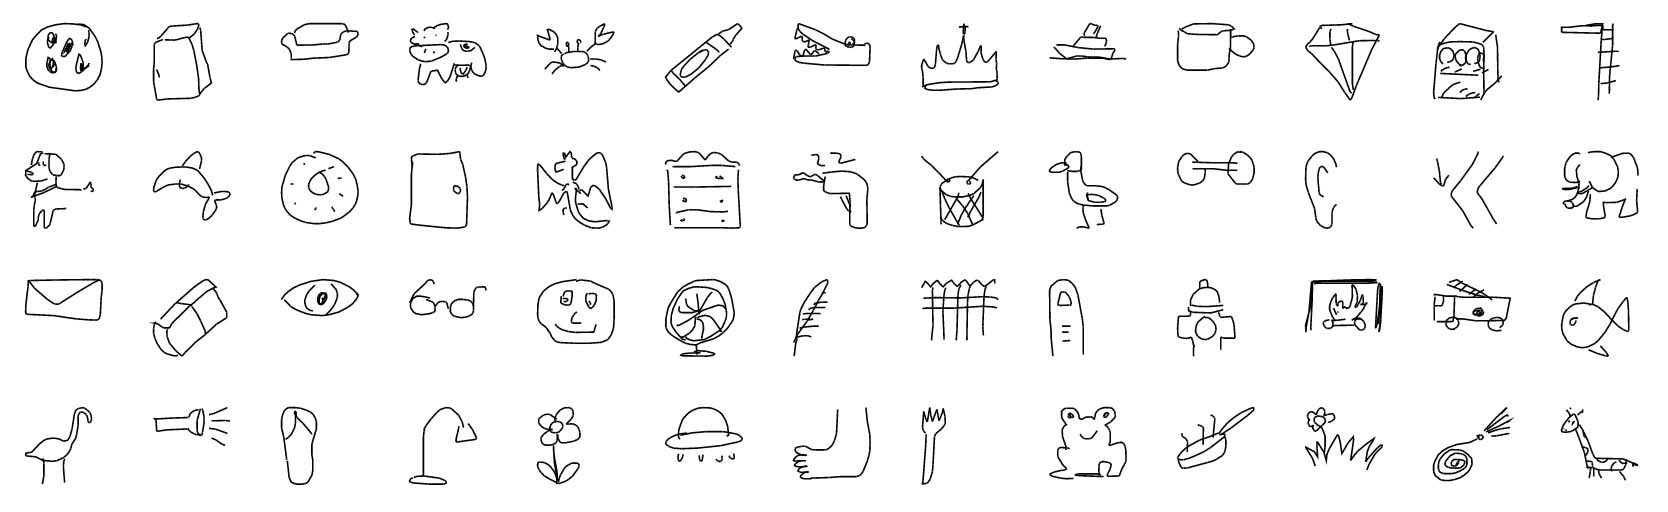
\includegraphics[height=150px,width=450px]{preview.jpg}
\end{center}
\caption{Exemple de dessins issus du dataset.}
\hrulefill
\end{figure}

\paragraph{Reconnaissance de dessins} Le modèle utilisé pour reconnaître les dessins est un CNN (Convolutionnal Neural Network) construit et entrainé avec la bibliothèque Keras. Il prend en input des "thumbnails" (ou miniatures en français) qui sont des images réduites à la taille de 28 × 28 pixels. 

\paragraph{Génération de dessins} Ce modèle sera un RNN (Recurrent Neural Network) qui sera entrainé avec la bibliothèque \href{https://magenta.tensorflow.org/}{Magenta} basée elle-même sur TensorFlow.

\section{Réalisation et difficultés rencontrées}

\subsection{Serveur Web et pages}

Le serveur web se lance en local à l'adresse {\tt localhost:3000}. Nous proposons un système de salon où l'utilisateur doit saisir un pseudo puis peut inviter des amis à le rejoindre. Nous avons réalisé un tableau blanc permettant aux utilisateurs de simplement pouvoir dessiner et effacer son dessin.

L'une des difficultés est la découverte du fonctionnement de Node.js et d'Express, notamment le fonctionnement interne du serveur et le routing.

\subsection{Construction modèle et entrainement}

\paragraph{Tâches réalisées} Nous avons réussi à construire et entraîner sur une vingtaine de classes (nous avons sélectionné les animaux du dataset pour faire des tests, nous ferons un choix définitif des classes plus tard), un modèle Keras à reconnaitre des dessins. Il a pour le moment un accuracy d'environ 75-80 \%. Nous pouvons aussi l'exporter et l'importer pour l'utiliser ailleurs.

\paragraph{Apprentissage du Python et de TensorFlow} La première grande difficulté est la découverte du Machine Learning et des bibliothèques en python dédiées. C'est un domaine assez vaste et complexe dont il n'est pas facile de commencer. Nous avons commencé par re-étudier les bases du Python puis les bases du machine learning avec TensorFlow et Keras. Le dataset a été utilisé dans de nombreux projets de recherche, d'art ou des projets universitaires. Il y a assez de documentation en libre-service pour étudier et utiliser le dataset mais paradoxalement, il y a très peu de ressources complètes sur comment construire et utiliser concrètement le dataset.

De plus, c'est très compliqué de comprendre certains messages d'erreur. Nous sommes parfois restés bloqués à cause de messages d'erreurs ambigus pendant assez longtemps.

\paragraph{Entrainement} Un autre gros problème est aussi l'entrainement des modèles. Cela prends des heures de télécharger et formater les données puis d'entrainer un modèle. Surtout quand le notebook crash par manque de RAM ou juste qu'il y a une erreur d'exécution. Nous avons fait le choix d'utiliser Google Colab pour ces tâches.

\section{Aperçu des prochaines étapes}

\subsection{Connexion à un salon}

\begin{itemize}
    \item Nous allons ajouter une page qui consiste à créer un nouveau salon où nous allons lui générer un identifiant ou de rejoindre un salon en entrant un numéro d'identifiant spécifique. Il pourra y avoir plusieurs salons créés en même temps, l'utilisateur doit pouvoir inviter ses amis dans son salon. Les utilisateurs devront être capables de voir qui est connecté au salon en temps réel.
    \item Nous devrons améliorer le salon en faisant fonctionner le bouton "COPIER LE LIEN" où une URL permettant de se connecter au salon sera copié sur le presse-papier.
    \item Les utilisateurs auront deux rôles, celui d'invité et celui du chef du salon. Seul le chef du salon pourra lancer la partie du jeu.
\end{itemize}

\subsection{Page de dessin}

\begin{itemize}
    \item Nous améliorerons la page de dessin pour qu'elle ait le comportement que nous voulons : quand on s'y connecte, un timer de 10 secondes se lance, le joueur alors dessiner. Une fois les 10 secondes écoulées, le dessin est renvoyé au serveur et le joueur et redirigé vers la manche suivante.
    \item Nous devrons créer la liste des mots qui s'afficheront en dessous du tableau de dessin. Il s'agit du mot que l'utilisateur devra dessiner et devra être sélectionné aléatoirement et envoyé à tous les joueurs.
\end{itemize}

\subsection{Accès aux pages}

Nous devrons vérifier, à chaque requête vers des pages du jeu, que l'utilisateur est bien dans une partie existante et en cours, et qu'il est bien à la bonne partie.

\subsection{Modèles}

\begin{itemize}
    \item Il va falloir améliorer les performances du modèle de reconnaissance ainsi que de l'entrainer avec de nouvelles classes.
    \item La prochaine étape sera de manipuler et d'entrainer le modèle de Magenta afin de pouvoir générer des dessins.
\end{itemize}
\end{document}